\chapter{Metaprogramming in Kotlin}\label{chapter:metaprogramming}
A typical program computation can be summarized as follows: it reads data as input, computes that data and generates an output. Metaprograms \cite{metaprogramming_introduction} are able to take as input another program, sometime even itself, manipulate it and return it with a modified behavior.\newline
Metaprogramming in Kotlin is a powerful feature that allows for the manipulation and generation of code at compile time. The possible benefits of this technique are:
\begin{itemize}
    \item Code generation: it generates repetitive or boilerplate code automatically, reducing the amount of code that needs to be written and maintained by hand. Consequently, this can increase code readability and maintainability, as well as reduce the risk of introducing bugs or errors;
    \item Readability: it provides a higher level of abstraction, allowing to abstract away complex logic and make code more readable and easier to understand. This can also help to simplify the implementation of complex algorithms and data structures;
    \item Reusability: by generating code automatically, it is possible reuse the same logic across multiple parts of applications, increasing overall code reuse and maintainability;
    \item Supports Domain-Specific Languages (DSLs): it enables to create custom, domain-specific languages (DSLs) that are optimized for specific tasks or use cases, which can help to simplify complex operations and make the code more readable and intuitive;
    \item Custom annotations: it allows creating custom annotations, which can be used to provide additional information about the code and to automate tasks such as code generation. This can improve code quality and make it easier to understand the intention behind the code.
\end{itemize}

\section{Metaprogramming techniques}
There are different techniques that can be used in Kotlin in order to create metaprograms. In the following sections they are going to be analyzed in details the main approaches provided by Kotlin, in order to give an overview of the possible alternatives when coming into terms with metaprogramming.

\subsection{Annotations}
Annotations \cite{annotation_documentation} in Kotlin are a type of metadata that can be added to provide additional information about the code, as well as to automate certain tasks.\newline
An annotation is represented by an \textbf{@} symbol followed by the annotation type.

To create a custom annotation in Kotlin, first it is necessary to declare the annotation type, using the \textbf{annotation} keyword in Kotlin, in the same way shown in the following code:
\begin{lstlisting}[caption={Example of creation of a custom annotation in Kotlin}, language=Kotlin, captionpos=b, label={code:kotlin_annotations_creation}]
annotation class MyAnnotation
\end{lstlisting}

Kotlin provides the option to use additional attributes by annotating the annotation class with \textbf{meta-annotation}. The alternatives of meta-annotation are:
\begin{itemize}
    \item \textbf{@Target}: it is used to specify the elements that can be annotated with the annotations, which can be classes, functions, properties and expressions;
    \item \textbf{@Retention}: it defines if an annotation is stored in the compiled class files and if it is visible at runtime using reflections;
    \item \textbf{@Repeatable}: it allows an annotation to be used on an element multiple times;
    \item \textbf{@MustBeDocumented}: it can be used when the annotation is part of a public API, and it must be included in the generated API documentation.
\end{itemize}

For example, this is a possible custom annotation that uses meta-annotation:
\begin{lstlisting}[caption={Example of custom annotation in Kotlin}, language=Kotlin, captionpos=b, label={code:kotlin_annotations_customization}]
@Target(AnnotationTarget.CLASS, AnnotationTarget.FUNCTION)
@Retention(AnnotationRetention.RUNTIME)
annotation class MyAnnotation
\end{lstlisting}
In this snippet of code, the \textbf{@Target} annotation specifies the elements that the annotation can be applied to, in this case either classes or functions. The \textbf{@Retention} annotation refers to the retention policy, which determines that the annotation is available at runtime.

Annotations can be used to provide metadata, such as the purpose of a function, the intended usage of a class, or the preferred behavior of a method. One possible use case is to use annotations to specify that a certain method should only be called on a background thread, or that a certain class is serializable.

Another feature provided by annotations, which is considered metaprogramming, is the possibility to used them to automate tasks, such as code generation. For example, annotations can be used to automatically generate code for serializing and deserializing objects.

It is possible to use the annotation in the code by placing the \textbf{@} symbol, followed by the annotation type before the element that is going to be annotated, such as a class, function, or property.\newline
The following snippet of code shows how to actually use a custom annotation, specifically the one created in Listing \ref{code:kotlin_annotations_customization}:
\begin{lstlisting}[caption={Example of usage of a custom annotation in Kotlin}, language=Kotlin, captionpos=b, label={code:kotlin_annotations_usage}]
@MyAnnotation
class MyClass

fun myFunction() {
    @MyAnnotation
    val myVariable = 42
}
\end{lstlisting}
In this example, the \textbf{MyAnnotation} annotation is applied to both a class and a variable. The annotations can be used by other code, either at compile time or at runtime, to provide additional information about the annotated elements.

\subsection{KSP}
KSP stands for \textbf{Kotlin Symbol Processing}, and it is an API that can be used to build lightweight compiler plugins \cite{ksp_documentation}. It offers an easier compiler plugin API that takes advantage of Kotlin's capabilities, but it keeps the learning curve low.

KSP has been developed as an alternative technology to kapt \cite{kapt_documentation}, which was used to allow annotation processing. Currently, kapt is in maintenance mode; it is being kept up-to-date with the new Kotlin and Java releases, without adding any features.\newline
In comparison to kapt, annotation processors that utilize KSP can be executed two times quicker.

Kotlin Symbol Processing is a feature of the Kotlin compiler that allows to manipulate the code at compile time by processing the symbols of the code. Because of that, it is possible to write metaprogramming code that analyze, transform, and generate other code, without the need to access the code at runtime.

This API allows processing Kotlin programs in a native way, with an understanding of Kotlin-specifc features, which includes extension functions, local functions and declaration-site variance. It models types explicitly, which enables type checking.

KSP models the structure of Kotlin programs, making class declarations, class members, functions and parameters accessible for processing, while elements such as if blocks and for loops are not.\newline
It can also be seen as a preprocessor framework, which makes a KSP plugin a symbol processor that follow three main steps:
\begin{enumerate}
    \item it analyzes the source program and its resources;
    \item it generates an output, which might be code or in another form;
    \item finally, the Kotlin compiler compiles the source program with the generated output.
\end{enumerate}

Differently from a typical compiler plugin, KSP restricts processors from modifying the source code, as it is considered read-only. This choice can be justified by the intention to prevent confusion that may arise from a plugin that modifies the language semantics.

When analyzing the source code, from the KSP perspective, it looks like this:
\begin{lstlisting}[caption={The source code from KSP perspective \cite{ksp_documentation}}, captionpos=b, label={code:ksp_source_code}]
KSFile
  packageName: KSName
  fileName: String
    declarations: List<KSDeclaration>
      KSClassDeclaration //class, interface, object
        simpleName: KSName
        qualifiedName: KSName
        containingFile: String
        typeParameters: KSTypeParameter
        parentDeclaration: KSDeclaration
        classKind: ClassKind
        primaryConstructor: KSFunctionDeclaration
        superTypes: List<KSTypeReference>
        //contains inner classes, functions, properties
        declarations: List<KSDeclaration>    
\end{lstlisting}
The Listing \ref{code:ksp_source_code} shows the data structure that is accessible using KSP. Specifically, in this code there is a class declaration (\textit{KSClassDeclaration}), and it is possible to get its name, type, parameters, inner declarations, and so on. This allows to have a complete overview of the code structure.

Two are the elements that KSP expects to be implemented: the \textbf{SymbolProcessorProvider} and the \textbf{SymbolProcessor}.\newline
The SymbolProcessorProvider interface is define like this:
\begin{lstlisting}[caption={SymbolProcessorProvider interface \cite{ksp_documentation}}, language=Kotlin, captionpos=b, label={code:symbol_processor_provider_interface}]
interface SymbolProcessorProvider {
    fun create(environment: SymbolProcessorEnvironment):
        SymbolProcessor
}
\end{lstlisting}
It must be implemented in order to be able to create a SymbolProcessor: because of that, the \textit{create} function is invoked when KSP creates an instance of the SymbolProcessor. The SymbolProcessorProvider is separated from the SymbolProcessor to give more freedom during the development.

This is the interface of the SymbolProcessor:
\begin{lstlisting}[caption={SymbolProcessor interface \cite{ksp_documentation}}, language=Kotlin, captionpos=b, label={code:symbol_processor_interface}]
interface SymbolProcessor {
    fun process(resolver: Resolver): List<KSAnnotated>
}
\end{lstlisting}
The only function that needs to be overridden is \textit{process}, which is typically used to read files and pass the elements to the visitors.\newline
The \textit{Resolver} is the entry point of the functionalities provided by KSP: it can be used, for example, to get all the files of the source code, the symbols with annotation, a class or a function declaration by name.\newline
As many other compiler related APIs, KSP supports the \textbf{visitor pattern}, allowing to examine each element in an object-oriented way.\newline
For example, this is an implementation of a visitor that inspects the declarations, and it collects the functions:
\begin{lstlisting}[caption={Visitor that collects function declarations \cite{ksp_documentation}}, language=Kotlin, captionpos=b, label={code:ksp_visitor}]
class FindFunctionsVisitor: KSTopDownVisitor<Unit, Unit>() {
    override fun visitFunctionDeclaration(
        function: KSFunctionDeclaration,
        data: Unit
    ) {
        functions.add(function.toString())
    }
}
\end{lstlisting}

In conclusion, one of the biggest strength of KSP is that it provides an API built on top of the compiler plugin: for this reason, it is able to hide the compiler changes, minimize maintenance efforts, and its API makes possible to implement a light-weight compiler plugin without the complexities and the knowledge required to create a real compiler plugin.\newline
On the other hand, since the goal of KSP is to be a simple solution for common problems, it comes with some limitations \cite{ksp_limitations}:
\begin{itemize}
    \item it can not examine expression-level information;
    \item it can not modify the source code, but it can only generate new code;
    \item it is not integrated with the IDE, meaning that the IDE has any information about the code generated.
\end{itemize}

\subsection{Kotlin compiler plugins}
Kotlin compiler plugins \cite{compiler_plugins_jetbrains} are a way to extend the functionality of the Kotlin compiler by adding custom processing to the compilation. This means that the compiler plugin code runs at compile-time, and, since this is a feature of \textit{kotlinc}, it only works on Kotlin source code.

Compiler plugins allow automating tasks and enforce coding standards. For example, they can be used to generate boilerplate code, such as accessor methods, or to enforce specific naming conventions or coding styles. Compiler plugins can also be used to perform code analysis and modification, such as adding custom checks and warnings, or refactoring the code automatically.

Kotlin compiler provides a powerful API, which makes it possible to even modify the internals of functions and classes. This enables to solve metaprogramming problems that were impossible using annotation processors, for example with KSP. Another advantage is that compiler plugins work on every Kotlin target, without having to write multiple plugin.

However, it is important to be aware of the potential downsides of using Kotlin compiler plugins. One of the main cons is that to write even a really simple plugin, it is necessary to have compiler background knowledge. Because of the high learning curve, it is important to consider very carefully if it is necessary to develop a plugin. The investment of time and work can be significant: other than understanding how a compiler plugin works, it is necessary to develop:
\begin{itemize}
    \item An IntelliJ plugin: whenever they are used synthetics members, such as functions that are going to be created by the plugin at compile time, the IntelliJ plugin is used to avoid error highlights, making it understand what is going on;
    \item A Gradle or Maven plugin: in order to make the user able to use and configure the compiler plugin;
    \item The actual compiler plugin.
\end{itemize}

Moreover, compiler plugins can slow down the compilation process and make it more complex. Additionally, they can have compatibility issues with different versions of the Kotlin compiler, and may require significant effort to maintain and update. It is also worth mentioning that because compiler plugins modify the behavior of the compiler, they can potentially introduce bugs and cause compatibility issues with other plugins.

Finally, another aspect that must be taken in consideration is the fact that the Kotlin compiler API is not documented. This means that working with it and understanding the function's behaviors is not an easy task, and it requires even more time.

A Kotlin compiler plugin architecture is organized as it can be seen in Figure \ref{fig:kotlin_compiler_plugin_architecture}.

\begin{figure}[!ht]
    \centering
    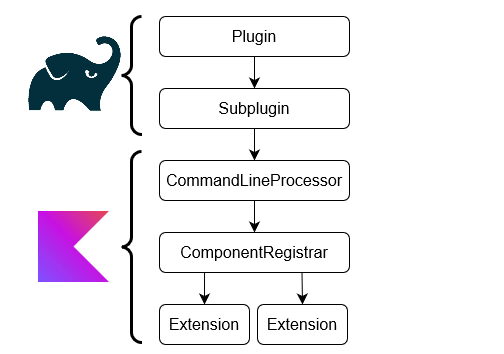
\includegraphics[scale=0.8]{document/chapters/2-metaprogramming/images/kotlin_compiler_plugin_architecture.png}
    \caption{The Kotlin compiler plugin architecture \cite{compiler_plugins_jetbrains}}
    \label{fig:kotlin_compiler_plugin_architecture}
\end{figure}

In the architecture can be distinguished two different modules: a Gradle module and a Kotlin module.

The \textbf{Gradle module} is a wrapper around the Kotlin module, and it is an entry point for Gradle. The Gradle module is composed by:
\begin{itemize}
    \item \textbf{plugin}: this part unrelated to Kotlin and it is based on the Gradle API. It provides an entry point from a build.gradle script, and it makes possible to configure the plugin via Gradle extensions;
    \item \textbf{subplugin}: this is the bridge that allows the interaction between Gradle and the Kotlin APIs. It reads the Gradle extension options, and it defines the compiler plugin's identifier, which is a unique key, in order to avoid collision with other plugins. The subplugin defines also the location of the compiler plugin, which is going to be used to download it at compile time. The location can be local or a Maven coordinate.
\end{itemize}

The \textbf{Kotlin module} is dived in three main parts:
\begin{itemize}
    \item \textbf{CommandLineProcessor}: the options created in the Gradle subplugin are loaded and used by the CommandLineProcessor. Whenever launching a Kotlin program, kotlinc is invoked: the arguments that are set in the subplugin are passed to the Kotlin compiler;
    \item \textbf{ComponentRegistrar}: it registers the extension components, which are going to be used when the project is compiled;
    \item \textbf{Extensions}: they are used to actually generate code. There are a lot of different extensions, which are used based on the use case.
\end{itemize}

Since the components of a plugin architecture are now explained from a general point of view, the focus is going to be now on the Kotlin module.
Specifically, the following sections are organized as follows: Section \ref{section:kotlin_ir} goes into details of the \textbf{IR} (\textbf{I}ntermediate \textbf{R}epresentation) that is the foundation that makes a compiler plugin possible, in Section \ref{section:compiler_plugin_basics} it is explained how to inspect and navigate Kotlin IR, in Section \ref{section:compiler_plugin_advaced} are covered advanced features, such as how to transform the Kotlin IR, and Section \ref{section:compiler_plugin_example} brings all together, showing the highlights of a working example of a simple Kotlin compiler plugin.

\subsubsection{Kotlin IR}\label{section:kotlin_ir}
The Kotlin compiler is organized in two parts: the \textit{frontend} is used to analyze the code, and the \textit{backend} is the one that generates the executables.\newline
Kotlin used to have three different backends: Kotlin/JVM, Kotlin/JS and Kotlin/Native. These backends were used to generate JVM byte code, JavaScript and LLVM IR, which is the representation for Kotlin Native.

When the Kotlin/Native backend was first developed, it was based on a new infrastructure, which used an internal representation for Kotlin code \cite{kotlin_ir_stabilization}. After its stabilization, Kotlin developers started to migrate the other two backends to the same representation. This allows to share the backend logic, and to have most of the feature and optimization done only once for all the targets. Moreover, the common backend infrastructure grant the possibility to create \textbf{multiplatform} compiler plugins.

The IR representation is an \textbf{abstract syntax tree} (\textbf{AST}). An AST \cite{ast_explanation} is a data structure that represents the abstract syntactic structure of a program. It is a tree representation of the source code, where each node in the tree corresponds to a construct in the source code. The nodes in the tree contain information about the construct, such as its type, location, and properties.\newline
For example, considering the following simple snippet of pseudocode:
\begin{lstlisting}[caption={Pseudocode of a simple assignment and expression}, language=Kotlin, captionpos=b, label={code:ast_pseudocode}]
if (a < b) {
    x = a + b
} else {
    x = a - b
}
\end{lstlisting}
The AST that is generated from the code structure of Listing \ref{code:ast_pseudocode} is shown in Figure \ref{fig:ast_pseudocode_example}.
\begin{figure}[!ht]
    \centering
    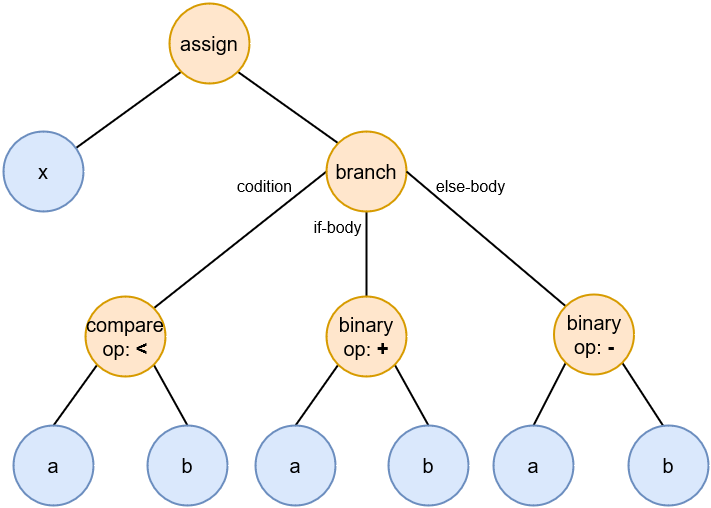
\includegraphics[scale=0.5]{document/chapters/2-metaprogramming/images/ast_pseudocode_example.png}
    \caption{The Abstract Syntax Tree of the source code in Listing \ref{code:ast_pseudocode}}
    \label{fig:ast_pseudocode_example}
\end{figure}
Each node in the tree describes a construct in the source code. The root node represents the assignment of the result of the \textit{branch} expression to the variable \textit{x}. The \textit{branch} defines the conditional construct, and it has three children: the \textit{condition}, the \textit{if-body} and the \textit{else-body}. Each of these blocks is represented by a separate subtree, with \textit{<}, \textit{+} and \textit{-} nodes representing the comparison, addition and subtraction operations, respectively. The nodes \textit{a} and \textit{b} are the variables, that are used as operands of these operations.\newline
The condition node is crucial, because it is used to decide whether to evaluate the \textit{if-body} or the \textit{else-body}.

The AST is generated by a parser, which takes the source code as input and constructs the tree representation based on the syntax rules of the language. Once the AST is generated, it can be used for various purposes, such as type checking, code analysis, optimization, and code generation.\newline
An AST provides a more abstract and structured representation of the source code compared to the raw source code. This makes it easier to analyze and manipulate the code, as well as to automatically generate code or perform other tasks. For example, compilers use the AST to perform optimizations, such as constant folding, dead code elimination, and inlining, before generating machine code.

Hence, \textbf{Kotlin IR} (Intermediate Representation) backend is a part of the Kotlin compiler that generates an intermediate representation of the Kotlin code. This is used as the input for the next stage of the compiler, which can be either the code generator or another intermediate representation.

The IR backend is designed to provide a high-level, platform-agnostic representation of the Kotlin code, making it easier to target different platforms and architecture. The IR code is optimized for use by the code generator, reducing the number of intermediate representations required, and allowing for better optimization.

Kotlin IR backend is an important part of the Kotlin compiler as it enables the compiler to target different platforms, such as the JVM, JavaScript, and Native code, while still providing a high-level representation of the code. This makes it easier to maintain and evolve the compiler and provides a more flexible way to target new platforms in the future.

\subsubsection{Basics}\label{section:compiler_plugin_basics}

\subsubsection{Advanced features}\label{section:compiler_plugin_advaced}
\subsubsection{Example}\label{section:compiler_plugin_example}
